%----------------------------------------------------------------------------
%----------------------------------------------------------------------------
%				    	SETUP
%----------------------------------------------------------------------------
%----------------------------------------------------------------------------

\documentclass[11pt]{article}

%----------------------------------------------------------------------------
%			  	   PACKAGES
%----------------------------------------------------------------------------

%%%%%%%%%%%%%%%%%%%%%%%
% 	  Packages
%%%%%%%%%%%%%%%%%%%%%%%

%% Fonts and Symbols
%% --------------------------
\usepackage{
	amsmath,			% math operators
	amssymb,			% math symbols
%	amsthm,				% theorem environment
	soul,				% strike through with \st{}
	textcomp,			% has \textuparrow
	xcolor,				% color!
%	xfrac,				% fancy fractions
}	

\definecolor{mygreen}{rgb}{0,0.6,0}
\definecolor{mygray}{rgb}{0.5,0.5,0.5}
\definecolor{mymauve}{rgb}{0.58,0,0.82}
\definecolor{darkblue}{rgb}{0,0,0.4}	

%% Graphics
%% --------------------
\usepackage{
	graphicx,			% allows insertion of images
	subfigure,			% allows subfigures (a), (b), etc.
	tikz,				% pretty pictures
}				
\graphicspath{ {graphics/} }	% (graphicx) relative path to graphics folder	
\usetikzlibrary{arrows, automata, calc, matrix, decorations.pathreplacing}			

%% Tables
%% --------------------------
\usepackage{
	booktabs,			% better tables, discourages vertical rulings
	multicol,			% allow multi columns
%			tocloft,			% finer control over TOC; enabled below due to subfigure conflict
}
%\usepackage[subfigure]{tocloft}
%\addtocontents{toc}{\cftpagenumbersoff{subsubsection}} % turn off subsubsection page numbers in ToC

%% Layout Alteration
%% --------------------------
\usepackage{			
%	caption,			% line breaks in captions with \\
%	changepage,			% change margins for PARTS of pages with (adjustwidth)
	fancyhdr,			% see config in LAYOUT AND STYLING
%	floatrow,			% multiple graphics, tables, etc in figure environment
	framed,				% nice boxes; used in Supervisor's Approval
%	fullpage,			% set full page margins
	geometry,			% change the margins for specific PAGES
%	lastpage,			% used with (fancyhdr)
	parskip,			% disable indents
	pdflscape,			% ???
	rotating,			% sideways figures
}
\geometry{						% specify page size options for (geometry)
	a4paper, 			% paper size
	hmargin=1in,		% horizontal margins
	vmargin=1in,		% vertical margins
}	


%% Units
%% --------------------------
\usepackage{
	siunitx,			% has S (decimal align) column type
}
\sisetup{input-symbols = {()},  % do not treat "(" and ")" in any special way
	group-digits  = false, 	% no grouping of digits
%	load-configurations = abbreviations,
%	per-mode = symbol,
}

%% Misc
%% --------------------------
\usepackage{
	enumitem,			% better control of enumerations, descriptions, etc
	listings,			% source code import and display
}

\lstset{ %
	language=verilog,				% the language of the code
	basicstyle=\footnotesize,       % the size of the fonts that are used for the code
	numbers=none,                   % where to put the line-numbers
	numberstyle=\tiny\color{mygray},% the style that is used for the line-numbers
	stepnumber=1,                   % the step between two line-numbers. If it's 1, each line
									% 	will be numbered
	numbersep=5pt,                  % how far the line-numbers are from the code
	backgroundcolor=\color{white},  % choose the background color. You must add \usepackage{color}
	showspaces=false,               % show spaces adding particular underscores
	showstringspaces=false,         % underline spaces within strings
	showtabs=false,                 % show tabs within strings adding particular underscores
	frame=single,	                % box the code [single, none]
	rulecolor=\color{black},        % if not set, the frame-color may be changed on line-breaks
									% 	within not-black text (e.g. commens (green here))
	tabsize=2,                      % sets default tabsize to 2 spaces
	captionpos=b,                   % sets the caption-position to bottom
	breaklines=true,                % sets automatic line breaking
	breakatwhitespace=false,        % sets if automatic breaks should only happen at whitespace
	title=\lstname,                 % show the filename of files included with \lstinputlisting;
									% 	also try caption instead of title
	keywordstyle=[1]\bfseries\color{darkblue},    % keyword style for mnemonics
	keywordstyle=[2]\bfseries\color{violet},	% keyword style for . mnemonics
	commentstyle=\color{mygreen},   % comment style
	stringstyle=\color{mymauve},    % string literal style
	escapeinside={\%*}{*)},         % if you want to add a comment within your code
	morekeywords={*,...}           	% if you want to add more keywords to the set
}

%----------------------------------------------------------------------------
%		     MACROS AND COMMANDS
%----------------------------------------------------------------------------

% Defines a new command for the horizontal lines, change thickness here
\newcommand{\HRule}{\rule{\linewidth}{0.5mm}} 

% override S column type with centered text column
\newcommand{\textcol}[1]{\multicolumn{1}{c}{#1}}


% Karnaugh maps! 
% http://tex.stackexchange.com/questions/140567/drawing-karnaughs-maps-in-latex
%isolated term
%#1 - Optional. Space between node and grouping line. Default=0
%#2 - node
%#3 - filling color
\newcommand{\implicantsol}[3][0]{
	\draw[rounded corners=3pt, fill=#3, opacity=0.3] ($(#2.north west)+(135:#1)$) rectangle ($(#2.south east)+(-45:#1)$);
}


%internal group
%#1 - Optional. Space between node and grouping line. Default=0
%#2 - top left node
%#3 - bottom right node
%#4 - filling color
\newcommand{\implicant}[4][0]{
	\draw[rounded corners=3pt, fill=#4, opacity=0.3] ($(#2.north west)+(135:#1)$) rectangle ($(#3.south east)+(-45:#1)$);
}

%group lateral borders
%#1 - Optional. Space between node and grouping line. Default=0
%#2 - top left node
%#3 - bottom right node
%#4 - filling color
\newcommand{\implicantlateral}[4][0]{
	\draw[rounded corners=3pt, fill=#4, opacity=0.3] ($(rf.east |- #2.north)+(90:#1)$)-| ($(#2.east)+(0:#1)$) |- ($(rf.east |- #3.south)+(-90:#1)$);
	\draw[rounded corners=3pt, fill=#4, opacity=0.3] ($(cf.west |- #2.north)+(90:#1)$) -| ($(#3.west)+(180:#1)$) |- ($(cf.west |- #3.south)+(-90:#1)$);
}

%group top-bottom borders
%#1 - Optional. Space between node and grouping line. Default=0
%#2 - top left node
%#3 - bottom right node
%#4 - filling color
\newcommand{\implicanttopbottom}[4][0]{
	\draw[rounded corners=3pt, fill=#4, opacity=0.3] ($(cf.south -| #2.west)+(180:#1)$) |- ($(#2.south)+(-90:#1)$) -| ($(cf.south -| #3.east)+(0:#1)$);
	\draw[rounded corners=3pt, fill=#4, opacity=0.3] ($(rf.north -| #2.west)+(180:#1)$) |- ($(#3.north)+(90:#1)$) -| ($(rf.north -| #3.east)+(0:#1)$);
}

%group corners
%#1 - Optional. Space between node and grouping line. Default=0
%#2 - filling color
\newcommand{\implicantcorners}[2][0]{
	\draw[rounded corners=3pt, opacity=.3] ($(rf.east |- 0.south)+(-90:#1)$) -| ($(0.east |- cf.south)+(0:#1)$);
	\draw[rounded corners=3pt, opacity=.3] ($(rf.east |- 8.north)+(90:#1)$) -| ($(8.east |- rf.north)+(0:#1)$);
	\draw[rounded corners=3pt, opacity=.3] ($(cf.west |- 2.south)+(-90:#1)$) -| ($(2.west |- cf.south)+(180:#1)$);
	\draw[rounded corners=3pt, opacity=.3] ($(cf.west |- 10.north)+(90:#1)$) -| ($(10.west |- rf.north)+(180:#1)$);
	\fill[rounded corners=3pt, fill=#2, opacity=.3] ($(rf.east |- 0.south)+(-90:#1)$) -|  ($(0.east |- cf.south)+(0:#1)$) [sharp corners] ($(rf.east |- 0.south)+(-90:#1)$) |-  ($(0.east |- cf.south)+(0:#1)$) ;
	\fill[rounded corners=3pt, fill=#2, opacity=.3] ($(rf.east |- 8.north)+(90:#1)$) -| ($(8.east |- rf.north)+(0:#1)$) [sharp corners] ($(rf.east |- 8.north)+(90:#1)$) |- ($(8.east |- rf.north)+(0:#1)$) ;
	\fill[rounded corners=3pt, fill=#2, opacity=.3] ($(cf.west |- 2.south)+(-90:#1)$) -| ($(2.west |- cf.south)+(180:#1)$) [sharp corners]($(cf.west |- 2.south)+(-90:#1)$) |- ($(2.west |- cf.south)+(180:#1)$) ;
	\fill[rounded corners=3pt, fill=#2, opacity=.3] ($(cf.west |- 10.north)+(90:#1)$) -| ($(10.west |- rf.north)+(180:#1)$) [sharp corners] ($(cf.west |- 10.north)+(90:#1)$) |- ($(10.west |- rf.north)+(180:#1)$) ;
}

%Empty Karnaugh map 4x4
\newenvironment{Karnaugh4x4}[2]%
{
	\begin{tikzpicture}[baseline=(current bounding box.north),scale=0.8]
	\draw (0,0) grid (4,4);
	\draw (0,4) -- node [pos=0.7,above right,anchor=south west] {#2} node [pos=0.7,below left,anchor=north east] {#1} ++(135:1);
	%
	\matrix (mapa) [matrix of nodes,
	column sep={0.8cm,between origins},
	row sep={0.8cm,between origins},
	every node/.style={minimum size=0.3mm},
	anchor=8.center,
	ampersand replacement=\&] at (0.5,0.5)
	{
		\& |(c00)| 00         \& |(c01)| 01         \& |(c11)| 11         \& |(c10)| 10         \& |(cf)| \phantom{00} \\
		|(r00)| 00             \& |(0)|  \phantom{0} \& |(1)|  \phantom{0} \& |(3)|  \phantom{0} \& |(2)|  \phantom{0} \&                     \\
		|(r01)| 01             \& |(4)|  \phantom{0} \& |(5)|  \phantom{0} \& |(7)|  \phantom{0} \& |(6)|  \phantom{0} \&                     \\
		|(r11)| 11             \& |(12)| \phantom{0} \& |(13)| \phantom{0} \& |(15)| \phantom{0} \& |(14)| \phantom{0} \&                     \\
		|(r10)| 10             \& |(8)|  \phantom{0} \& |(9)|  \phantom{0} \& |(11)| \phantom{0} \& |(10)| \phantom{0} \&                     \\
		|(rf) | \phantom{00}   \&                    \&                    \&                    \&                    \&                     \\
	};
}%
{
	\end{tikzpicture}
}

%Empty Karnaugh map 2x4
\newenvironment{Karnaugh2x4}[2]%
{
	\begin{tikzpicture}[baseline=(current bounding box.north),scale=0.8]
	\draw (0,0) grid (4,2);
	\draw (0,2) -- node [pos=0.7,above right,anchor=south west] {#2} node [pos=0.7,below left,anchor=north east] {#1} ++(135:1);
	%
	\matrix (mapa) [matrix of nodes,
	column sep={0.8cm,between origins},
	row sep={0.8cm,between origins},
	every node/.style={minimum size=0.3mm},
	anchor=4.center,
	ampersand replacement=\&] at (0.5,0.5)
	{
		\& |(c00)| 00         \& |(c01)| 01         \& |(c11)| 11         \& |(c10)| 10         \& |(cf)| \phantom{00} \\
		|(r00)| 0             \& |(0)|  \phantom{0} \& |(1)|  \phantom{0} \& |(3)|  \phantom{0} \& |(2)|  \phantom{0} \&                     \\
		|(r01)| 1             \& |(4)|  \phantom{0} \& |(5)|  \phantom{0} \& |(7)|  \phantom{0} \& |(6)|  \phantom{0} \&                     \\
		|(rf) | \phantom{00}  \&                    \&                    \&                    \&                    \&                     \\
	};
}%
{
	\end{tikzpicture}
}

%Empty Karnaugh map 2x2
\newenvironment{Karnaugh2x2}[2]%
{
	\begin{tikzpicture}[baseline=(current bounding box.north),scale=0.8]
	\draw (0,0) grid (2,2);
	\draw (0,2) -- node [pos=0.7,above right,anchor=south west] {#2} node [pos=0.7,below left,anchor=north east] {#1} ++(135:1);
	%
	\matrix (mapa) [matrix of nodes,
	column sep={0.8cm,between origins},
	row sep={0.8cm,between origins},
	every node/.style={minimum size=0.3mm},
	anchor=2.center,
	ampersand replacement=\&] at (0.5,0.5)
	{
		\& |(c00)| 0          \& |(c01)| 1  \\
		|(r00)| 0 \& |(0)|  \phantom{0} \& |(1)|  \phantom{0} \\
		|(r01)| 1 \& |(2)|  \phantom{0} \& |(3)|  \phantom{0} \\
	};
}%
{
	\end{tikzpicture}
}

%Defines 8 or 16 values (0,1,X)
\newcommand{\contingut}[1]{%
	\foreach \x [count=\xi from 0]  in {#1}
	\path (\xi) node {\x};
}

%Places 1 in listed positions
\newcommand{\minterms}[1]{%
	\foreach \x in {#1}
	\path (\x) node {1};
}

%Places 0 in listed positions
\newcommand{\maxterms}[1]{%
	\foreach \x in {#1}
	\path (\x) node {0};
}

%Places X in listed positions
\newcommand{\dontcare}[1]{%
	\foreach \x in {#1}
	\path (\x) node {X};
}


%----------------------------------------------------------------------------
%----------------------------------------------------------------------------
%				   DOCUMENT
%----------------------------------------------------------------------------
%----------------------------------------------------------------------------

\begin{document}

%----------------------------------------------------------------------------
%				    TITLE PAGE
%----------------------------------------------------------------------------

\begin{titlepage}

\center
 
% Header
\textsc{\LARGE University of Victoria}\\[1cm] 	% Name of your university/college
\textsc{\Large CENG 241}\\[0.5cm] 			% Major heading such as course name
\textsc{\large Digital Design I}\\[0.5cm] 		% Minor heading such as course title


% Lab Title
\HRule \\[0.4cm]
{\huge \bfseries Lab 7:  RAM System}\\[0.2cm] % Title of your document
\HRule \\[1.5cm]
 
 
%Lab Instructor Details
\begin{minipage}{0.7\textwidth}
\begin{flushleft} 

\large\emph{Instructor:} \\
Dr. Amirali \textsc{Baniasadi} \\
\vspace{12 pt}
\emph{Teaching Assistant:} \\
Grace \textsc{Hui}

\end{flushleft}
\end{minipage}
~
%% No content here, but it keeps the alignment of the instructor/TA
%% box correct.
%% Consider revising.
\begin{minipage}{0.1\textwidth}
\begin{flushright} \large
%Dr. Barbara \textsc{Sawicka} \\
\vspace{12 pt}
%\emph{Teaching Assistant:} \\
%Vahid \textsc{Moradi}
\end{flushright}
\end{minipage}\\[2cm]


% Lab members
\Large Yves \textsc{S\'{e}n\'{e}chal}
\large V00213837	\\
\Large Tyler \textsc{Stephen}
\large V00812021	\\
A01 - B03\\[1.5cm] 


% Date
{\large July 27, 2015}\\ % Date, change the \today to a set date if you want to be precise

% Logo
\begin{figure}[b]	 % put logo at bottom of the page
	\centering
	\includegraphics[scale=0.3]{UVic_logo}
\end{figure}

\end{titlepage}

%----------------------------------------------------------------------------
%				    BODY
%----------------------------------------------------------------------------

\section{Introduction}

This lab will detail the construction of a RAM system with the ability to store and retrieve 4-bit datawords. A 4-bit counter will generate sequential addresses, a tri-state buffer will control the data input line and a 4-bit register will store the retrieved data from RAM (see Figure \ref{fig:controller}). The focus of this lab will be on the construction of the controller. The purpose of the controller is to ensure that each component in the RAM system is configured properly in the correct sequence needed for reading or writing to RAM.

\begin{figure}[htpb]
	\centering
	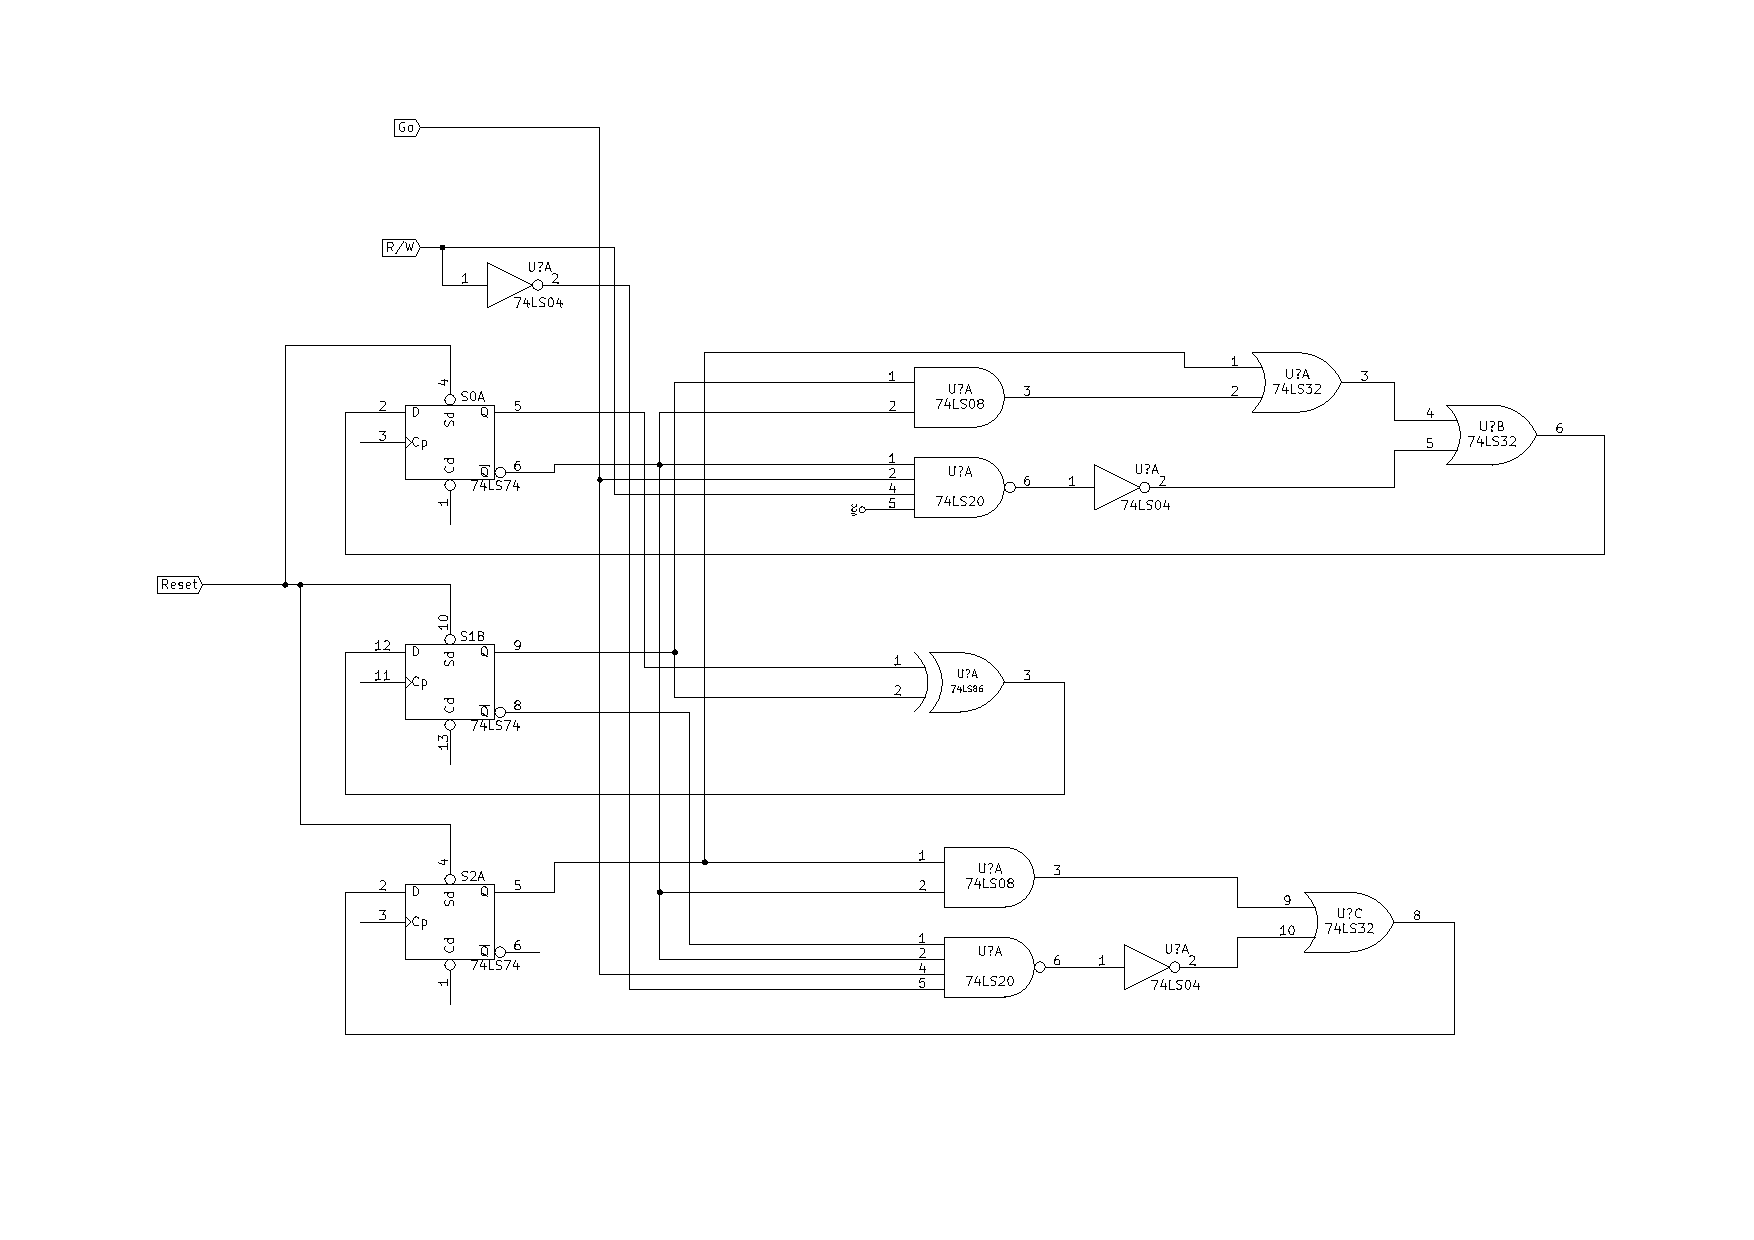
\includegraphics[scale=0.5]{controller}
	\caption{RAM controller and memory system}
	\label{fig:controller}
\end{figure}

\section{Discussion}\label{sec:discussion}

The RAM, buffer and register are connected to each other via an address bus. In order for the RAM system to function properly, it is essential that there is only one correct ``path'' for the data to take on the bus. By changing the operating mode of the RAM, register and buffer, the controller changes the path for the data.

When the system is powered on and reset it enters an idle state where both the RAM and register are ``closed'' (their inputs are set to high impedance) and the buffer is passing the selected dataword to the address bus. Based on user input, the read or write cycles can be activated.

To write to RAM:
\begin{enumerate}
 
 	 \item RAM I/O is configured as an input and is no longer high impedance
	 \item a clock cycle passes to prevent timing problems
 	 \item the counter is incremented to a new address and the RAM returns to high impedance
	 \item the system returns to idle
	  
\end{enumerate}

\newpage
To read from RAM:

\begin{enumerate}
 
 	 \item RAM I/O is configured as an output and the buffer is set to high impedance
 	 \item the register reads the RAM output from the bus
 	 \item the counter is incremented, the RAM returns to high impedance, the register returns to high impedance and cycles the previous RAM output and the buffer outputs a new dataword to the bus
 	 \item the system returns to idle
	  
\end{enumerate}

This process is represented as a state machine in Figure \ref{fig:state}.

\subsection{Timing considerations}

The read and write timing diagrams, shown in Figure \ref{fig:read-timing} and Figure \ref{fig:write-timing} respectively, indicate that the moment in which the data is valid is offset from moment where the address is valid; the data is valid after the address is valid. The access time and hold time for the read operation and write operation respectively can be attributed to the RAM's internal delay of \SI{85}{\nano\second} maximum. However, this does not pose a problem with a manual clock, but could become a nuisance should high-frequency clock be used.

\begin{figure}[htpb]
	\centering
	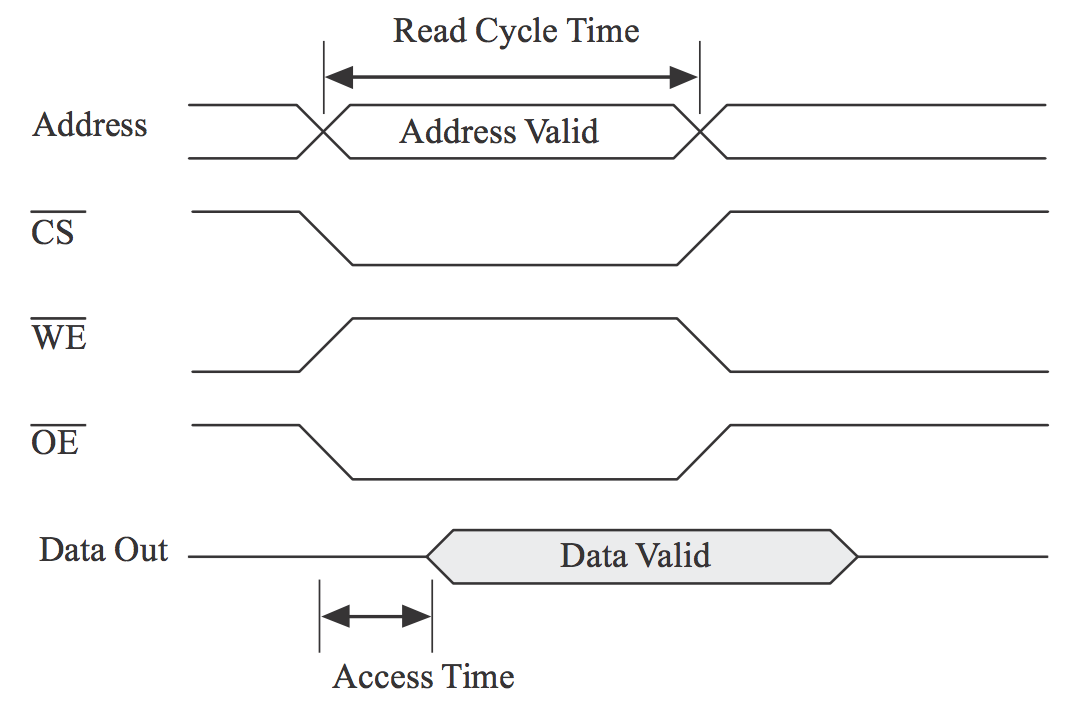
\includegraphics[scale=0.5]{read}
	\caption{Timing diagram for the RAM read operation}
	\label{fig:read-timing}
\end{figure}

\begin{figure}[htpb]
	\centering
	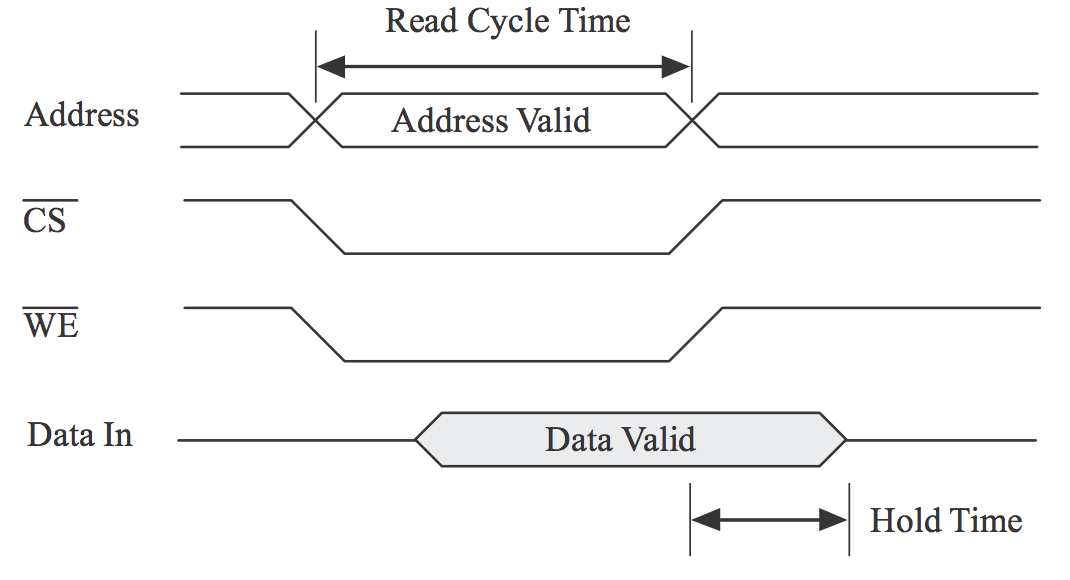
\includegraphics[scale=0.5]{write}
	\caption{Timing diagram for the RAM write operation}
	\label{fig:write-timing}
\end{figure}

\section{RAM controller design process}
\subsection{State diagram}

The state diagram of the RAM controller is shown in Figure \ref{fig:state} (note, \textuparrow\; signifies a clock rising edge). The system was designed as a Moore machine with the transition tables displayed in figure \ref{table:transition-moore}. 

\begin{figure}[htpb]
	\centering
	\begin{tikzpicture}
	[>=stealth', shorten >= 1pt, auto, node distance=4cm]
	\node[state, initial, align=center]	(a) []					{$(a)$\\$\overline{Read}=0$};
	\node[state, align=center](b) [above left of=a]	{$(b)$\\$\overline{OE}=0$\\$\overline{WE}=1$};
	\node[state, align=center]			(c) [above right of=b]	{$(c)$\\$Load=1$};
	\node[state, align=center]			(d) [right of=a]	{$(d)$\\$Incr=1$};
	\node[state, align=center](e) [below left of=a]	{$(e)$\\$\overline{OE}=0$\\$\overline{WE}=0$};
	\node[state, align=center](f) [below right of=e]{$(f)$\\Load into \\ RAM};
	
	\path[->]
	(a) edge [bend left]	node [right, align=left, pos=0.7, yshift=5]	{$Go=1$\\$R/\overline{W}=1$}		(b)
	edge [loop above]	node [above]	{$Go=0$}		(a)
	(b)	edge [bend left]	node			{\textuparrow}	(c)
	(c)	edge [bend left]	node			{\textuparrow}	(d)
	(d) edge 				node [right, yshift=15]{\textuparrow}	(a)
	(a) edge [bend right]	node [right, align=left, pos=0.7, yshift=-5]	{$Go=1$\\$R/\overline{W}=0$}		(e)
	(e)	edge [bend right]	node [left, yshift=-10]{\textuparrow}	(f)
	(f)	edge [bend right]	node [right, yshift=-10]{\textuparrow}	(d)
	;
	
	\draw [decorate,decoration={brace,amplitude=10pt,mirror},xshift=-4pt,yshift=0pt]
	(6.5,1.0) -- (6.5,6.5) node [black,midway,xshift=2.5cm,align=left] 
	{Read from \\ RAM};
	
	%		\draw [decorate,decoration={brace,amplitude=10pt},xshift=-4pt,yshift=0pt]
	%		(10.5,0.95) -- (10.5,-0.95) node [black,midway,xshift=0.5cm,align=left] 
	%		{Steady \\ state};
	
	\draw [decorate,decoration={brace,amplitude=10pt},xshift=-4pt,yshift=0pt]
	(6.5,-1.0) -- (6.5,-6.5) node [black,midway,xshift=0.5cm,align=left] 
	{Write to \\ RAM};
	\end{tikzpicture}
	\caption{State diagram for the RAM controller}
	\label{fig:state}
\end{figure}	

\newpage

\begin{figure}[htpb]
	\centering
	\subfigure[State enumeration]
	{
		\begin{tabular}{c | c c c }
			State & $S_2$ & $S_1$ & $S_0$ \\
			\hline
			$a$ & 0 & 0 & 0 \\
			$b$ & 0 & 0 & 1 \\
			$c$ & 0 & 1 & 0 \\
			$d$ & 0 & 1 & 1 \\
			$e$ & 1 & 0 & 0 \\
			$f$ & 1 & 0 & 1 \\
			 -  & 1 & 1 & 0 \\
			 -  & 1 & 1 & 1 \\
		\end{tabular}
	}
	\subfigure[Next state]
	{
		\begin{tabular}{c c c c c | c c c}
			$S_2$ & $S_1$ & $S_0$ & $Go$ & $R/\overline{W}$ & $S_2^+$ & $S_1^+$ & $S_0^+$ \\
			\hline
			0 & 0 & 0 & 0 & 0 & 0 & 0 & 0 \\
			0 & 0 & 0 & 0 & 1 & 0 & 0 & 0 \\
			0 & 0 & 0 & 1 & 0 & 1 & 0 & 0 \\
			0 & 0 & 0 & 1 & 1 & 0 & 0 & 1 \\
			0 & 0 & 1 & 0 & 0 & 0 & 1 & 0 \\
			0 & 0 & 1 & 0 & 1 & 0 & 1 & 0 \\
			0 & 0 & 1 & 1 & 0 & 0 & 1 & 0 \\
			0 & 0 & 1 & 1 & 1 & 0 & 1 & 0 \\
			0 & 1 & 0 & 0 & 0 & 0 & 1 & 1 \\
			0 & 1 & 0 & 0 & 1 & 0 & 1 & 1 \\
			0 & 1 & 0 & 1 & 0 & 0 & 1 & 1 \\
			0 & 1 & 0 & 1 & 1 & 0 & 1 & 1 \\
			0 & 1 & 1 & 0 & 0 & 0 & 0 & 0 \\
			0 & 1 & 1 & 0 & 1 & 0 & 0 & 0 \\
			0 & 1 & 1 & 1 & 0 & 0 & 0 & 0 \\
			0 & 1 & 1 & 1 & 1 & 0 & 0 & 0 \\
			1 & 0 & 0 & 0 & 0 & 1 & 0 & 1 \\
			1 & 0 & 0 & 0 & 1 & 1 & 0 & 1 \\
			1 & 0 & 0 & 1 & 0 & 1 & 0 & 1 \\
			1 & 0 & 0 & 1 & 1 & 1 & 0 & 1 \\
			1 & 0 & 1 & 0 & 0 & 0 & 1 & 1 \\
			1 & 0 & 1 & 0 & 1 & 0 & 1 & 1 \\
			1 & 0 & 1 & 1 & 0 & 0 & 1 & 1 \\
			1 & 0 & 1 & 1 & 1 & 0 & 1 & 1 \\
			1 & 1 & 0 & 0 & 0 & - & - & - \\
			1 & 1 & 0 & 0 & 1 & - & - & - \\
			1 & 1 & 0 & 1 & 0 & - & - & - \\
			1 & 1 & 0 & 1 & 1 & - & - & - \\
			1 & 1 & 1 & 0 & 0 & - & - & - \\
			1 & 1 & 1 & 0 & 1 & - & - & - \\
			1 & 1 & 1 & 1 & 0 & - & - & - \\
			1 & 1 & 1 & 1 & 1 & - & - & - \\
		\end{tabular}
	}
	\caption[figurename=Table]{Transition tables for the Moore machine}
	\label{table:transition-moore}
\end{figure}


From here three karnaugh maps were used to resolve the next states $S_2^+$, $S_1^+$, and $S_0^+$. Their state equations are shown below.

\begin{align*}
	S_2^+ &= S_2 S_0^{\prime} + S_1^{\prime} S_0^{\prime}\; Go\; R/\overline{W}\\
	S_1^+ &= S_1\; \text{XOR}\; S_0 \\
	S_0^+ &= S_2 + S_1 S_0^{\prime} + S_0^{\prime}\; Go\; R/\overline{W} \\
\end{align*}

\newpage

We were able to reduce the complexity of the controller by eliminating two outputs from the controller in Figure \ref{fig:controller}. $\overline{CS}$ was set to LOW peramently and the $\overline{Reset}$ line was externalized from the state machine and made asynchronous. The state outputs are summarized in table \ref{table:state_output}. Five karnaugh maps were needed to resolve their state equations which are shown below.

\begin{align*}
	\overline{OE} &= S_1^{\prime} S_0^{\prime} + S_1 S_0 \\
	\overline{WE} &= S_2^{\prime} \\
	Load &= S_1 S_0^{\prime} \\
	\overline{Read} &= S_1 + S_2^{\prime} S_0 \\
	Incr &= S_1 S_0 \\
\end{align*}

\begin{table}
	\centering
		\begin{tabular}{c c c | c c c c c }
			$S_2$ & $S_1$ & $S_0$ & $\overline{OE}$ & $\overline{WE}$ & $Load$ & $\overline{Read}$ & $Incr$\\
			\hline
			0 & 0 & 0 & 1 & 1 & 0 & 0 & 0 \\
			0 & 0 & 1 & 0 & 1 & 0 & 1 & 0 \\
			0 & 1 & 0 & 0 & 1 & 1 & 1 & 0 \\
			0 & 1 & 1 & 1 & 1 & 0 & X & 1 \\
			1 & 0 & 0 & X & 0 & 0 & 0 & 0 \\
			1 & 0 & 1 & X & 0 & 0 & 0 & 0 \\
			1 & 1 & 0 & - & - & - & - & - \\
			1 & 1 & 1 & - & - & - & - & - \\
		\end{tabular}
	\caption{State output}
	\label{table:state_output}
\end{table}

Although the lab manual made it seem necessary to include state $f$ to accommodate timing delays from the RAM, our work in the lab found that the RAM output would appear in the registers in state $e$. This suggests that $f$ and $e$ could be condensed and the number of states reduced by one. However, we would still need three flip-flops to implement the five remaining states.

\subsection{Controller logic}

The logic of the RAM controller was implemented with D flip-flops. Figure \ref{fig:schematic-controller} shows the design of the state machine and Figure \ref{fig:schematic-output} shows the logic for generating the output.

\begin{figure}[htpb]
	\centering
	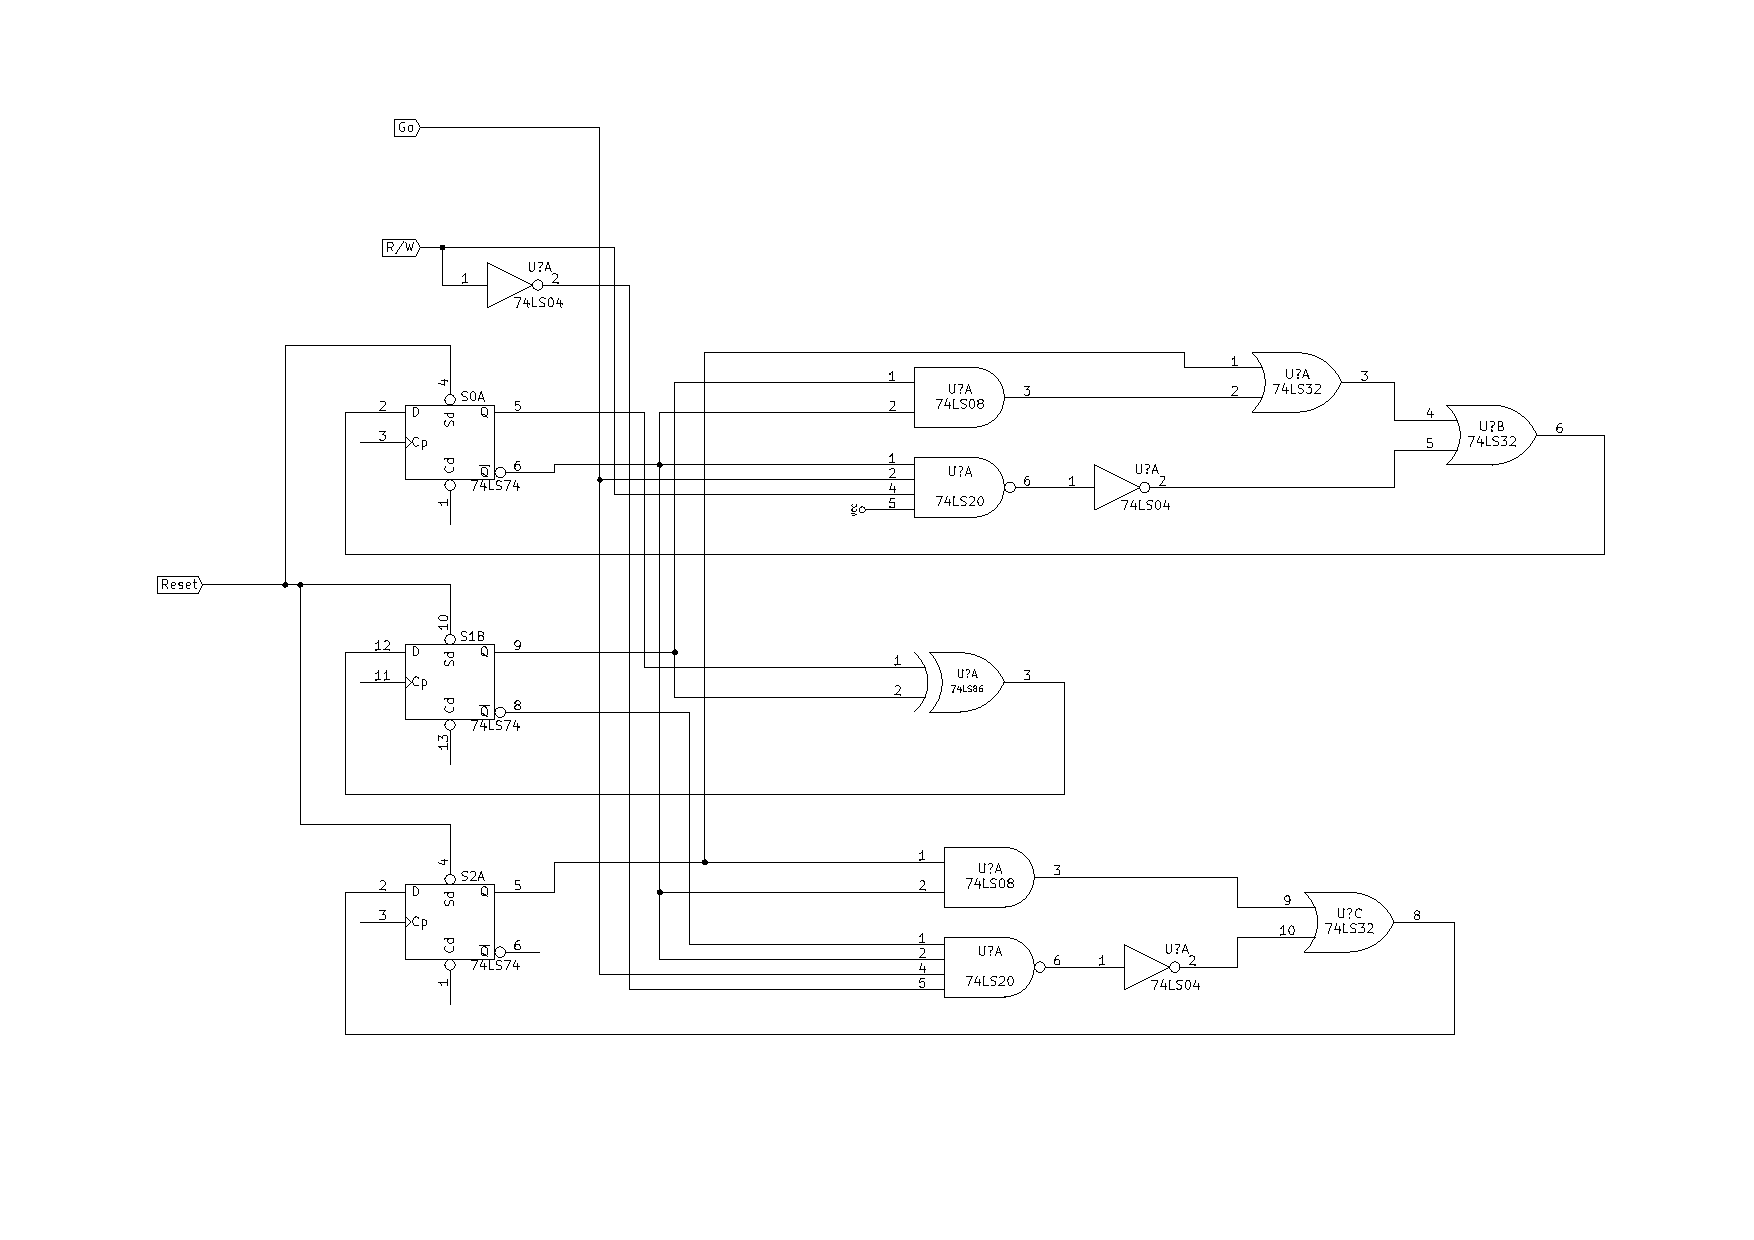
\includegraphics[scale=0.5]{controller.pdf}
	\caption{RAM controller state machine}
	\label{fig:schematic-controller}
\end{figure}

\begin{figure}[htpb]
	\centering
	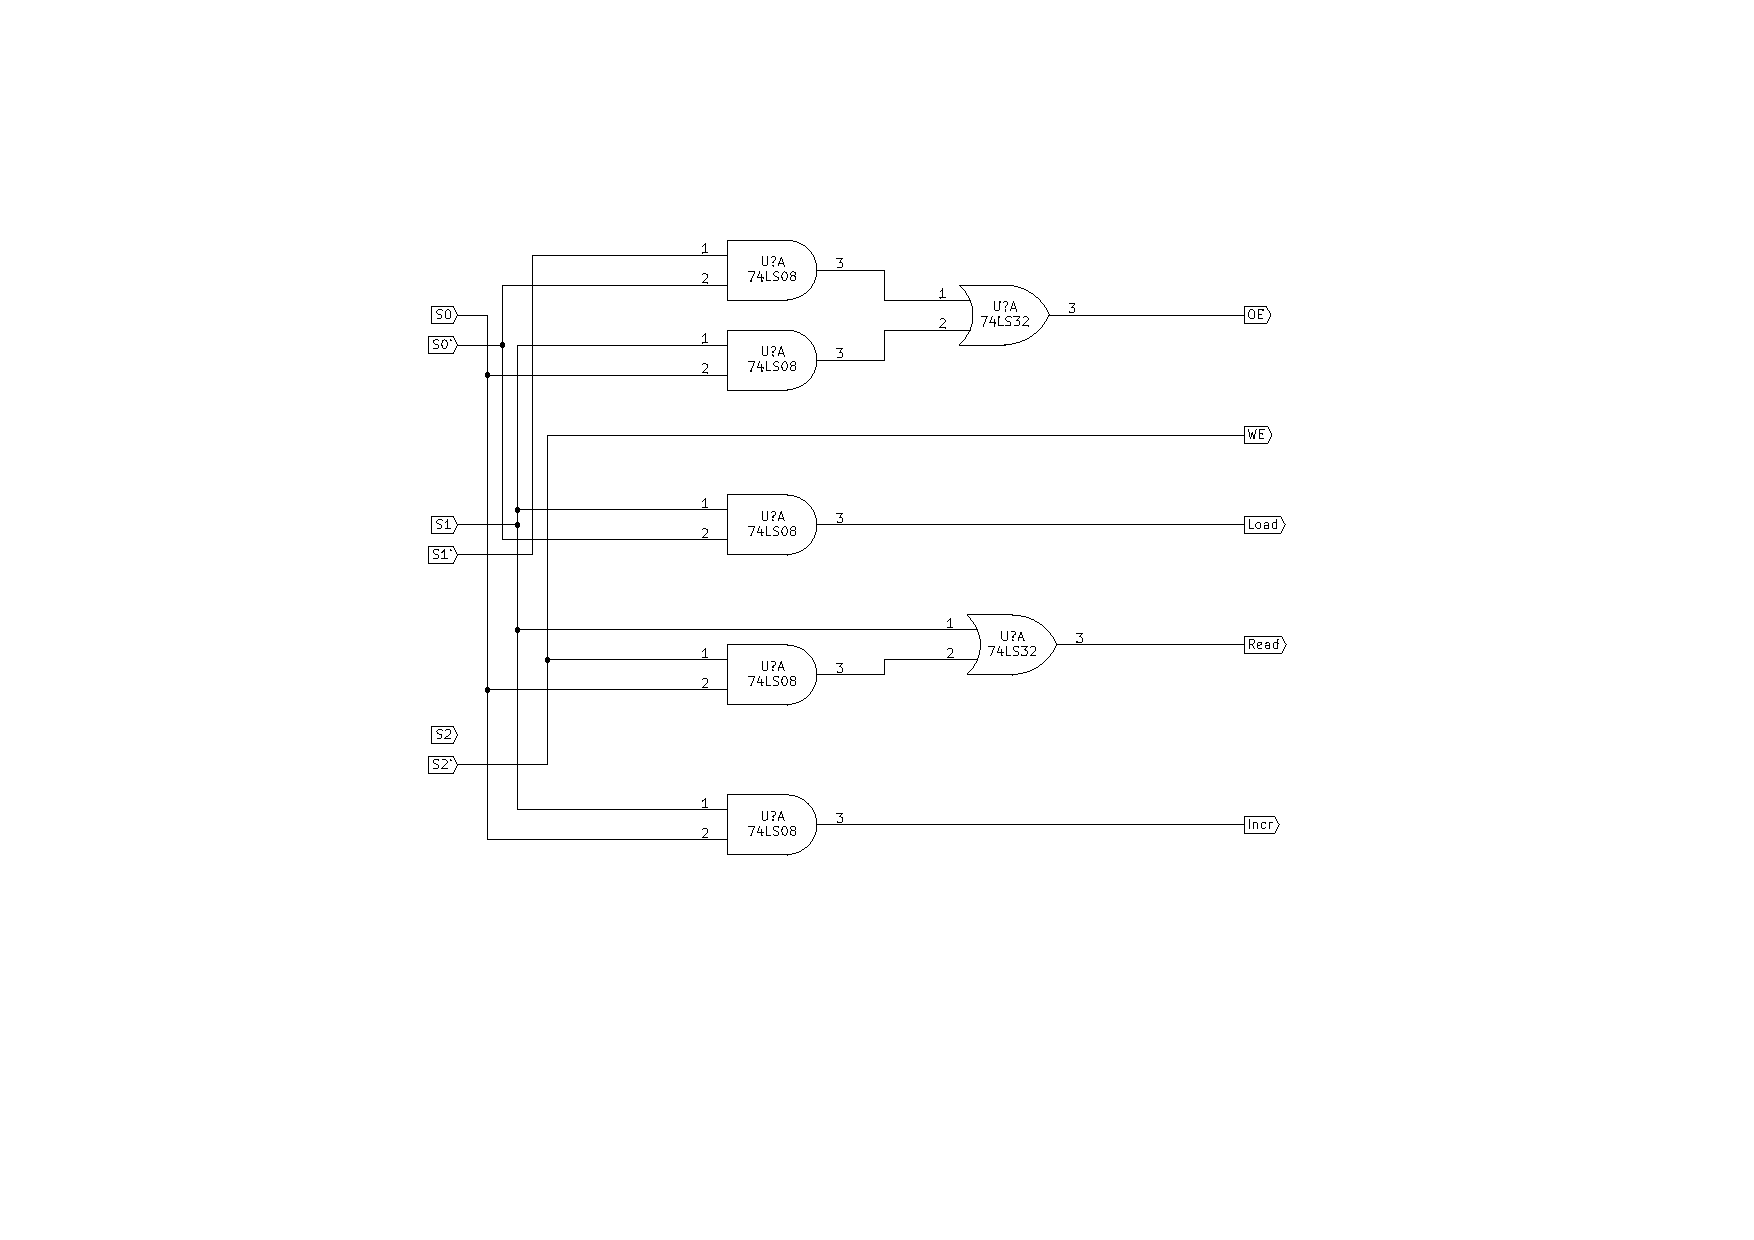
\includegraphics[scale=0.5]{output.pdf}
	\caption{RAM controller output}
	\label{fig:schematic-output}
\end{figure}

\section{Conclusion}

A functioning 4-bit RAM controller was built using D flip-flops and some external logic. The system had a 4-bit counter which determined the address of the data. Four LEDs displayed the present address, while, when in read mode, four other LEDs revealed the stored data at that address. 

\end{document}